\documentclass{mwrep}

% Polskie znaki
\usepackage{polski}
\usepackage[utf8]{inputenc}
\usepackage[T1]{fontenc}
\usepackage{lmodern}
\usepackage{indentfirst}

% Strona tytułowa
\usepackage{pgfplots}
\usepackage{siunitx}
\usepackage{paracol}

% Pływające obrazki
\usepackage{float}
\usepackage{svg}
\usepackage{graphicx}

% table of contents refs
\usepackage{hyperref}
\usepackage{cleveref}
\usepackage{booktabs}
\usepackage{listings}


\SendSettingsToPgf
\title{\bf Projekt układu sterowania stanowiska INTECO TCRANE \vskip 0.1cm}
\author{Krystian Guliński \\ Jakub Sikora \\ Konrad Winnicki }
\date{\today}
\pgfplotsset{compat=1.15}	
\begin{document}

\makeatletter
\renewcommand{\maketitle}{\begin{titlepage}
		\begin{center}{
				\LARGE {\bf Politechnika Warszawska}}\\
            \vspace{0.4cm}
            \leftskip-0.9cm
            {\LARGE {\bf \mbox{Wydział Elektroniki i Technik Informacyjnych}}}\\
            \vspace{0.2cm}
            {\LARGE {\bf \mbox{Instytut Automatyki i Informatyki Stosowanej}}}\\
            
            \vspace{5cm}
            \leftskip-1.5cm
			{\bf \Huge \mbox{Systemy automatyki DCS i SCADA} \vskip 0.1cm}
		\end{center}
		\vspace{0.1cm}

		\begin{center}
			{\bf \LARGE \@title}
		\end{center}

		\vspace{10cm}
		\begin{paracol}{2}
			\addtocontents{toc}{\protect\setcounter{tocdepth}{1}}
			\subsection*{Zdający:}
			\bf{ \Large{ \noindent\@author \par}}
			\addtocontents{toc}{\protect\setcounter{tocdepth}{2}}

			\switchcolumn \addtocontents{toc}{\protect\setcounter{tocdepth}{1}}
			\subsection*{Prowadzący:}
			\bf{\Large{\noindent mgr. inż. Andrzej \\ Wojtulewicz}}
			\addtocontents{toc}{\protect\setcounter{tocdepth}{2}}

		\end{paracol}
		\vspace*{\stretch{6}}
		\begin{center}
			\bf{\large{Warszawa, \@date\vskip 0.1cm}}
		\end{center}
	\end{titlepage}
}
\makeatother
\maketitle

\tableofcontents


\chapter{Opis stanowiska}
\label{Opis}

\section{Stanowisko TCRANE}
\label{Opis::TCRANE}
Trójwymiarowy model laboratoryjnego modelu dźwigu ilustruje strukturę współczesnego 
żurawia, skutecznie odwzorowuje stosunek wielkości do maksymalnego podnoszonego 
ładunku. Obiekt jest wielowejściowym i wielowyjściowym systemem wyposażonym w dedykowane
czujniki do mierzenia przemieszczeń i kątów.\\
\indent Stanowisko laboratoryjne T-Crane posiada 5 enkoderów inkrementalnych. Trzy z nich
mierzą położenie elementów napędzanych przez silniki. Dwa z nich znajdują się na karetce
dźwigu i przedstawiają aktualne wychylenie obciążenia od pionu.

\begin{figure}[H]
    \label{Opis::TCRANE::Stanowisko}
    \centering
    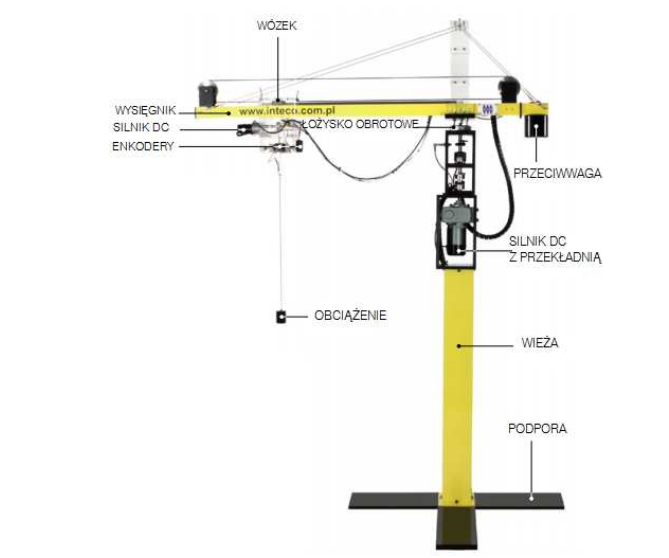
\includegraphics[scale=0.5]{tcrane.png}
    \caption{Stanowisko laboratoryjne TCRANE}
\end{figure}

W ramach projektu laboratoryjnego, mieliśmy wysterować ramię dźwigu w dwóch płaszczyznach:

\begin{itemize}
    \item obrót kolumny dźwigu (wieży)
    \item ruch wózka wzdłuż ramienia
\end{itemize}

\section{Enkodery inkrementalne}
\label{Opis::Enkodery}
Enkoder (przetwornik położenia) służy do pomiaru położenia. W powyższej wersji
mamy do czynienia z przetwornikiem obrotowym. Zatem możemy dzięki niemu określić
położenie kątowe wokół osi. Jeżeli podłączymy go do liniowego układu przeniesienia napędu
możemy określić położenie liniowe wyrażane w odległości.\\
\indent Do określenia kierunku potrzebujemy dwóch sygnałów (tzw.
fazy A i B).Do określenia pozycji wykorzystujemy dwa wejścia do zliczania 
impulsów z fazy A i B. Wykrywanie kierunku jest wykonywane
automatycznie w sterowniku. Przy pomocy mechanizmu sprzętowych liczników możemy w
dowolnym momencie odczytać aktualne położenie enkodera. W pamięci
sterownika pozycja będzie przedstawiona w odpowiednim rejestrze 32 bitowym.\\
\indent Zliczanie impulsów odbywa się za pomocą liczników \emph{High Speed Counter}.
Pozycja zadawana w procentach jest programowo zamieniana na impulsy enkodera 
według następującego wzoru:

$$ I = \frac{STPT * MAX}{100\%}$$

Dla wózka jeżdżącego wzdłuż ramienia $$MAX_{wozek} = 9000,$$
natomiast dla wieży $$MAX_{wieza} = 2300$$

\section{Opis wejść i wyjść obiektu}
\label{Opis::IO}

\subsection{Wejścia cyfrowe}
\label{Opis::IO::Input}

\begin{table}[H]
    \centering
    \begin{tabular}{|p{0.1\linewidth}|p{0.6\linewidth}|}
	\hline
	Wejście & Opis \\ \hline
	X0 & Enkoder inkrementalny, fala A, oś X              \\ \hline
	X1 & Enkoder inkrementalny, fala B, oś X                   \\ \hline
	X2 & Enkoder inkrementalny, fala A, oś Y 		         \\  \hline
	X3 & Enkoder inkrementalny, fala B, oś Y            \\ \hline
	X4 & Enkoder inkrementalny, fala A, oś AX 		         \\  \hline
    X5 & Enkoder inkrementalny, fala B, oś AX           \\ \hline
    X6 & Enkoder inkrementalny, fala A, oś AY 		         \\  \hline
    X7 & Enkoder inkrementalny, fala B, oś AY            \\ \hline
    X10 & Enkoder inkrementalny, fala A, oś Z  		         \\  \hline
    X11 & Enkoder inkrementalny, fala B, oś Z            \\ \hline
    X12 & Wyłącznik krańcowy, oś Z 		         \\  \hline
    X13 & Wyłącznik krańcowy, oś X 		         \\  \hline
    X14 & Wyłącznik krańcowy, oś Y 		         \\  \hline
    X15 & Flaga limitu temperatury, oś Z 		         \\  \hline
    X16 & Flaga limitu temperatury, oś Y 		         \\  \hline
    X17 & Flaga limitu temperatury, oś X 		         \\  \hline
	\end{tabular}
    \caption{Wejścia instalacji INTECO TCRANE}
\end{table}
\newpage

\subsection{Wyjścia cyfrowe}
\label{Opis::IO::Output}

\begin{table}[H]
    \centering
    \begin{tabular}{|p{0.1\linewidth}|p{0.6\linewidth}|}
	\hline
    Wejście & Opis \\ \hline
    Y0 & Sygnał PWM dla silnika DC, oś X  \\  \hline
	Y1 & Sygnał PWM dla silnika DC, oś Z  \\ \hline
	Y2 & Sygnał PWM dla silnika DC, oś Y  \\ \hline
	Y3 & Hamulec silnika DC, oś Z 		  \\  \hline
	Y4 & Wybór kierunku obrotów silnika DC, oś Z         \\ \hline
	Y5 & Hamulec silnika DC, oś Y 		  \\  \hline
	Y6 & Wybór kierunku obrotów silnika DC, oś Y         \\ \hline
    Y7 & Hamulec silnika DC, oś X 		  \\  \hline
    Y10 & Wybór kierunku obrotów silnika DC, oś X         \\ \hline
	\end{tabular}
	\caption{Wyjścia instalacji INTECO TCRANE}
\end{table}

\chapter{Sterownik PLC}
\label{PLC}

\section{Konfiguracja sprzętowa}
\label{PLC::Konfiguracja}

\subsection{Ethernet}
\label{PLC::Konfiguracja::Ethernet}

W celu umożliwienia komunikacji sterownika z komputerem PC, odpowiednio skonfigurowaliśmy
połączenie w sieci Ethernet. Komunikacja odbywa się za pomocą protokołu SLMP (SeamLess 
Message Protocol) na porcie 1280. 

\begin{figure}[H]
    \label{PLC::Konfiguracja::Ethernet::Window}
    \centering
    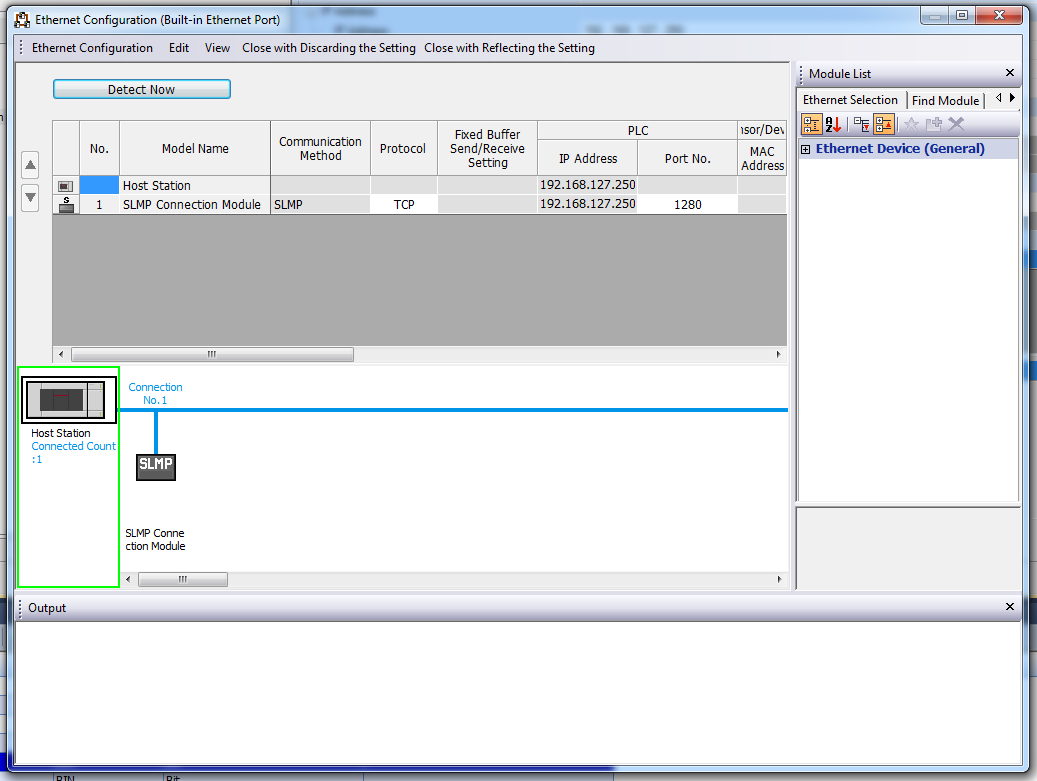
\includegraphics[scale=0.3]{ethernet.png}
    \caption{Konfiguracja komunikacji w sieci Ethernet w systemie GX Works3}
\end{figure}

\subsection{Analog}
\label{PLC::Konfiguracja::Analog}

Obsługa wejść analogowych została przedstawiona jako jedno z kryterium oceny projektu.
Niestety, stanowisko INTECO TCRANE nie zawiera żadnych wejść i wyjść analogowych. 

\subsection{High Speed Counter}
\label{PLC::Konfiguracja::HIOEN}

Odczyt z enkoderów inkrementalnych odbywał się za pomocą specjalnych liczników \emph{High Speed
Counter}. Skonfigurowaliśmy dwa kanały CH1 oraz CH5 do odczytu pozycji wózka oraz obrotu wieży. 
Wartość pozycji wózka odczytywaliśmy spod adresu \texttt{SD4500} a wartość pozycji kątowej wieży 
spod adresu \texttt{SD4620}.

\newpage

\begin{figure}[H]
    \label{PLC::Konfiguracja::HIOEN::WindowCH1}
    \centering
    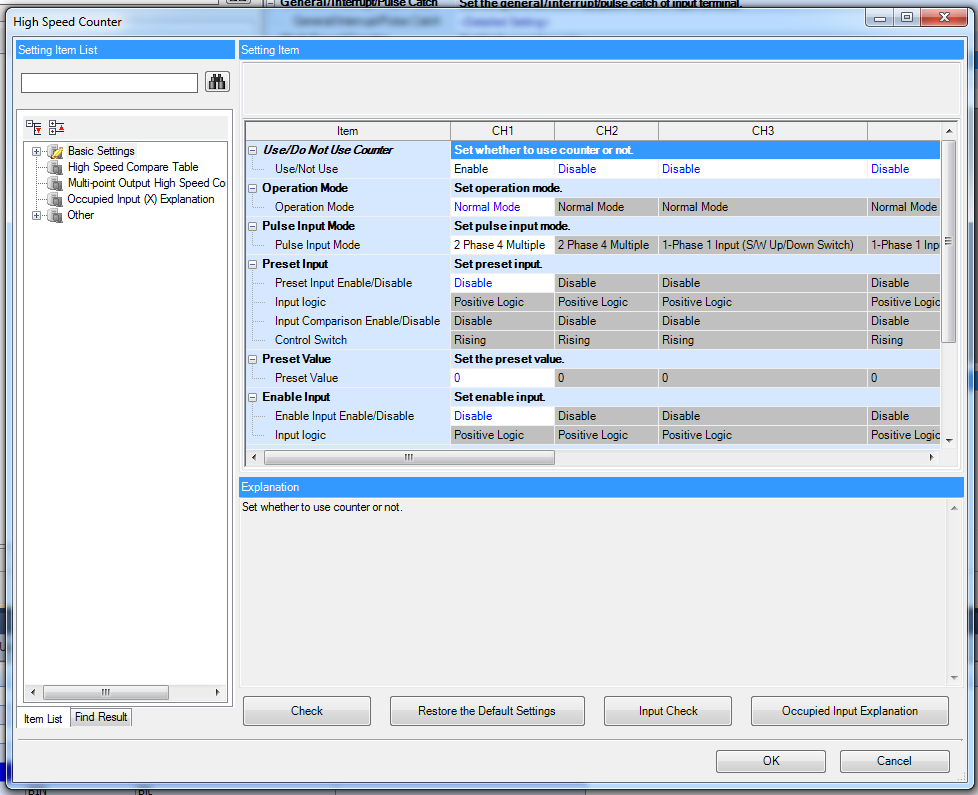
\includegraphics[scale=0.3]{hioen.png}
    \caption{Okno konfiguracji kanału \emph{CH1} High Speed Counters w systemie GX Works3}
\end{figure}

\begin{figure}[H]
    \label{PLC::Konfiguracja::HIOEN::WindowCH5}
    \leftskip-1.5cm
    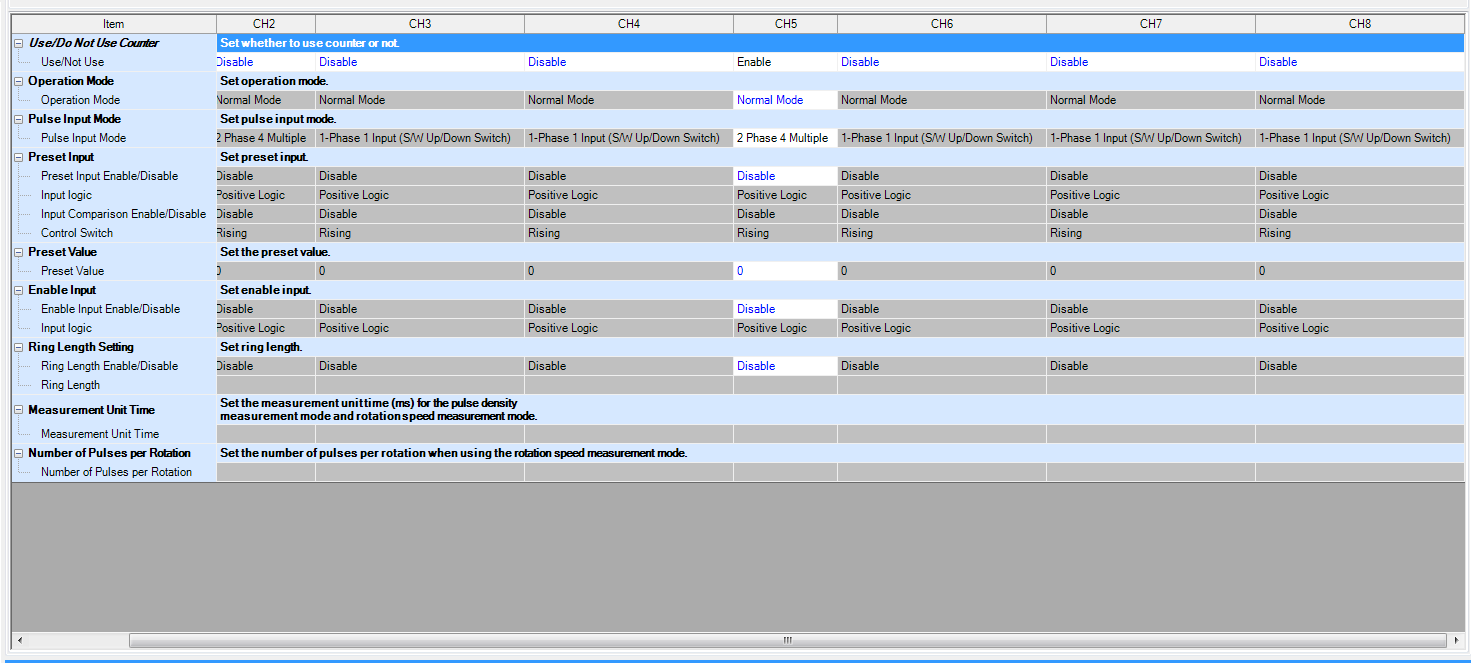
\includegraphics[scale=0.3]{hioen2.png}
    \caption{Okno konfiguracji kanału \emph{CH5} High Speed Counters w systemie GX Works3}
\end{figure}


\subsection{Wyjścia PWM}
\label{PLC::Konfiguracja::PWM}



\newpage
\section{Mechanizm labeli}
\label{PLC::Labels}

\section{Skalowanie i bazowanie}
\label{PLC::Bazowanie}

\section{Obsługa I/O cyfrowych}
\label{PLC::IOCyfrowe}

\section{PID}
\label{PLC::PID}

\section{Tryb sterowania ręcznego}
\label{PLC::Reka}

\section{Zabezpieczenia ruchów krańcowych}
\label{PLC::Krancowki}

\section{Język ST}
\label{PLC::ST}

\chapter{Realizacja w systemie MAPS}
\label{MAPS}

\section{Panel operatorski}
\label{MAPS::PanelOperatorski}

\section{Sterowanie auto/ręka}
\label{MAPS::AutoReka}

\section{Nastawy regulatorów}
\label{MAPS::Nastawy}

\section{Wykresy}
\label{MAPS::Wykresy}

\end{document}